\documentclass{article}

% preamble
% --------
\usepackage{graphicx}
\usepackage[font={footnotesize,sf}]{caption}
\usepackage[hidelinks]{hyperref}

\usepackage{amsmath}
\DeclareMathOperator{\erf}{erf}
\DeclareMathOperator{\lngamma}{\ln\!\Gamma}
\DeclareMathOperator{\Tr}{Tr}
\DeclareMathOperator*{\argmax}{arg\,max}

\usepackage{amssymb}
\usepackage{bm}

\usepackage{bbm}
\renewcommand{\P}{\mathbb{P}} % Probability
\newcommand{\E}{\mathbb{E}} % Expectation
\newcommand{\R}{\mathbb{R}} % Reals

\usepackage{amsthm}
\newtheorem{theorem}{Theorem}
\newtheorem{lemma}{Lemma}
\newtheorem{prop}{Proposition}
% --------


\title{\LaTeX{} template}
\author{You \and me}

\begin{document}

\maketitle

\section*{Introduction}\label{sec:intro}

\begin{prop}\label{prop:evo}
Evolution is awesome.
\end{prop}
\begin{proof}
  See \cite{darwin1909origin} and Figure~\ref{fig:darwin} in \nameref{sec:results}.
\end{proof}

\section*{Results}\label{sec:results}

As shown in Figure~\ref{fig:darwin}, Charles Darwin rocked hard---really hard.
This finding is used to prove Proposition~\ref{prop:evo}.

% WSD: DALLE image generation inspired by Andy Kern's tweet https://twitter.com/pastramimachine/status/1536354513627381760?s=20&t=NGXiPZuz9rHWdMvJpMoCrw
\begin{figure}[h]
 \centering
 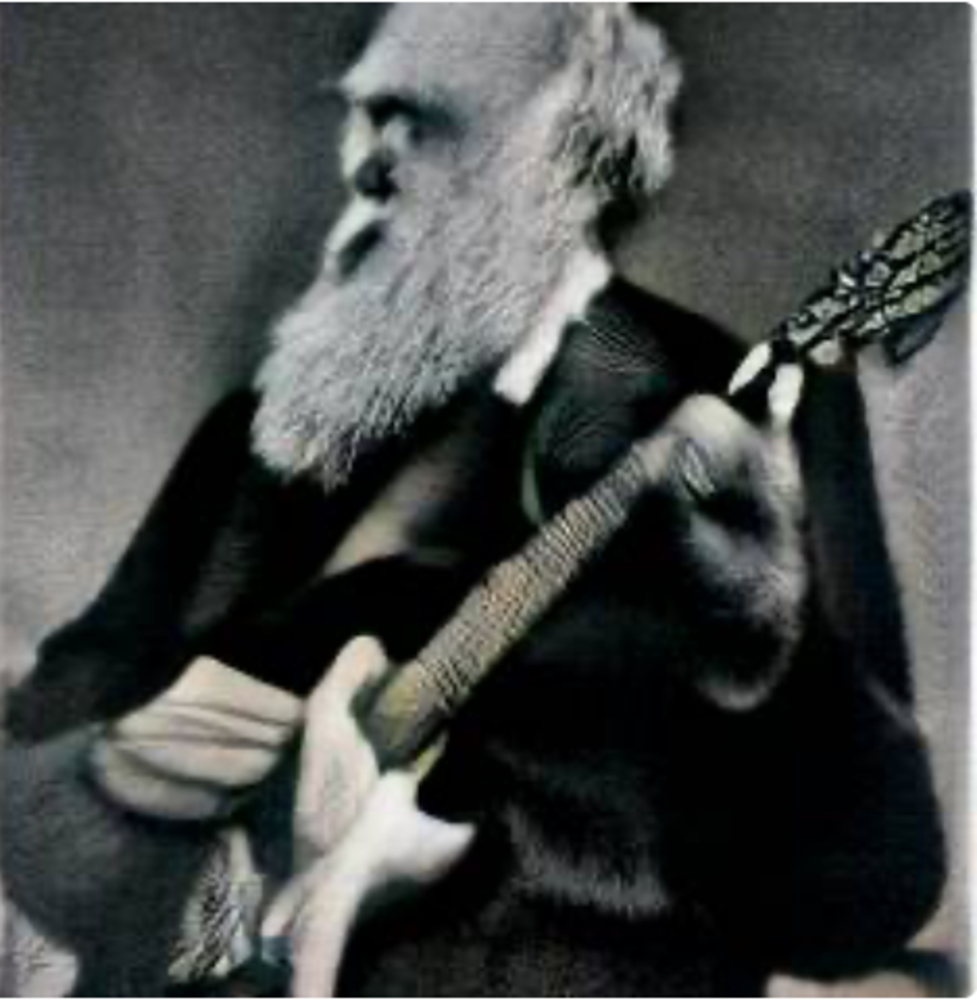
\includegraphics[width=0.3\textwidth]{figures/darwin-rock}
 \caption{Archival photograph of Charles Darwin playing his electric guitar.}
 \label{fig:darwin}
\end{figure}


\bibliographystyle{plain}
\bibliography{references}

\end{document}
